\documentclass{article}
\usepackage{minted}
\usepackage[utf8]{inputenc}
\usepackage[french]{babel}
\usepackage{mathtools}
\usepackage{graphicx} 
\usepackage{hyperref}
\usepackage{xcolor}
\usepackage{hyperref}
\definecolor{bg}{HTML}{282828}
\usemintedstyle{monokai}
\hypersetup{
    colorlinks=true,
    linkcolor=blue,
    filecolor=magenta,      
    urlcolor=cyan,
}
\urlstyle{same}

\title{Rapport projet PFA 2018-2019}
\date{\today}
\author{Lam NGUYEN THIET
\and Kenyu KOBAYASHI}
\begin{document}
\maketitle
\tableofcontents
\newpage
\newpage
\section{Introduction}
Ce projet implémente un jeu dans le langage OCAML, en utilisant les paradigmes fonctionelles (en majorité), impératives, orientée objet.

\section{Le jeu}
\subsection{Commandes}
Nous n'avons pas eu le temps d'implémenter l'interaction avec la souris. Les commandes se font intégralement
au clavier.
\begin{itemize}
    \item \texttt{Z S Q D}, pour bouger la caméra, resp., en haut, bas, gauche droite.
    \item \texttt{W C}, pour zoomer, resp. dézoomer
    \item \texttt{Entrée} pour sélectionner un allié
    \item \texttt{Y U I O P} pour sélectionner un action, resp. utiliser la bombe nucléaire, utiliser un pack de soin, ramasser un item, attaquer, se déplacer.
    \item Les fléches permettent de déplacer le curseur.
\end{itemize}

Pour effectuer une action, il faut faire :
\begin{enumerate}
    \item Sélectionner un personnage
    \item Sélectionner une action
    \item Sélectionner une destination
    \item Appuyer sur entrée pour confirmer
    
\end{enumerate}
\subsection{But}
Le but du jeu est de détruire les factions ennemies. Pour se faire, il suffit de tuer toutes leur unités.

Vous commencez avec 5 unités, les ennemis commencent avec 2 et une ville chacun. Ils peuvent apparaître à l'infini. 
Le seul moyen de détruire une ville est d'envoyer la bombe nucléaire. La stratégie est donc de saisir le plus rapidement les bombes nucléaires pour
détruire les villes aussitôt que possible.

\subsection{Factions}
Il y a 3 factions dans le jeu. Les cagoulés, les vert et les bleus. Vous contrôlez les bleus.

\subsection{Unités}
Il existe deux types d'unités.

\begin{itemize}
    \item Le soldat est l'unité de base. Elle peut se déplacer, attaquer et récupérer des items.
    \item La ville permet de faire apparaître des soldats. Cette unité est très importante car si on la perd, on ne peut plus produire de soldat.
\end{itemize}

\subsection{Items}
Il existe deux items.

\begin{itemize}
    \item Le pack de soin régénére la vie des unités. Il est possible d'avoir plus de points de vie que l'on avait au départ.
    \item La bombe nucléaire détruit tout dans un rayon de 3 cases.
\end{itemize}

\subsection{Plateau du jeu}
Le plateau est une grille d'hexagone. La carte est une île deserte dans l'océan avec des biômes variés.

\subsubsection{Type de cases}
Il y a 3 types de cases. A l'heure actuelle, elle ne sont que cosmétiques, par la suite elle peuvent avoir un impact sur l'efficacité de combat de tel unité de
tel faction, mais par manque de temps je n'ai pas pu les faire.

Il y a la neige, le desert et l'herbe.

\subsubsection{Caractèristiques du terrain}
En plus du biome, il y a des caractèristiques sur le terrain pour chaque case.

\begin{itemize}
    \item Les forêts et les collines coûtent plus cher pour le movement.
    \item Les montagnes et les lacs sont des obstacles ne peuvent pas être traversés.
\end{itemize}

\subsection{Tour par tour}
Le jeu se déroule en tour par tour, similaire au jeu \textit{Civilization}. C'est d'ailleurs
sur quoi je me suis inspiré pour le jeu.

\subsubsection{Mouvement}

Chaque unité a un nombre de movement. Lorsqu'il se déplace d'une case, il consomme $n$ points selon la case sur laquelle il atterit.
Dans le jeu, les soldats sont les seuls à pouvoir se déplacer. Les villes ne peuvent pas.

\subsubsection{Attaque}
Pour tuer les autres unités il faut les attaquer. Encore une fois de manière analogue à \textit{Civilization},
les unités disposent d'une force d'attaque et d'une force de défense.

Par la suite, $src$ et $dst$ représente respectivement l'unité qui attaque et l'unité
qui défend.

Lorsque deux unités s'attaquent, les nouveaux point de vie se calculent de cette manière : 

\begin{align}
    healthpoints_{dst,new} &= max \{0,healthpoints_{dst,old} - strength_{attack,src}\} \\
    healthpoints_{src,new} &= max \{0,healthpoints_{src,old} - strength_{defense,dst}\}
\end{align}

Et leurs nouvelles positions : 
\begin{align}
     x_{dst,new},y_{dst,new} &=
     \begin{cases}
        \texttt{null},\texttt{null} & \text{si } healthpoints_{dst_,new} = 0 \text{,}\\
        x_{dst,old},y_{dst,old} & \text{sinon.} 
     \end{cases} \\
     x_{src,new},y_{src,new} &=
     \begin{cases}
        \texttt{null},\texttt{null} & \text{si } healthpoints_{src,new} = 0 \text{,}\\
        x_{dst,old},y_{dst,old} & \text{si } healthpoints_{dst_,new} = 0 \text{,}\\
        x_{src,old},y_{src,old} & \text{sinon.} 
     \end{cases}
\end{align}

\subsection{Intelligence Artificielle}
Les IA sont assez simple. De base, elles se déplacent au hasard.
Si elles rencontrent un ennemi, elle va se diriger vers cet ennemi en priorité. Si il y a un
autre ennemi elles s'attaquent, même si ce n'était pas l'ennemi en priorité.

En dessous d'un certain seuil, les IA vont chercher à fuire et chercher un pack de soin. Mais si il y a un ennemi
tout prés, elles vont se suicider et attaquer cet ennemi, car elles savent qu'elles vont mourir et vont préférer attaquer 
pour donner une chance à leur alliés.

Sinon, en mode patrouille, si elles voient une bombe nucléaire, elles la prennent et l'utilise sur un ennemi au hasard.
\section{Répartition du travail}
\subsection{NGUYEN THIET}
\begin{itemize}
    \item Gestion des appels à la bibliothéque SDL ( \textit{e.g.,} gestion du render, chargement des textures, initialisation
    du windows, \textit{etc.} )
    \item Dessins (tuiles, caractèristiques de terrain, soldats, ville, interfaces, fond d'écran, titre, items, effets spéciaux)
    \item Définition des boucles du menu et du jeu et le retour que chaque boucle passe entre elles.
    \item Boucle principale. Gestion d'un type \texttt{context}, comment le mettre à jour et comment récupérer informations contenus pour avancer le jeu dans le temps
    \item Définition du type des \texttt{unités} et les méthodes associées
    \item Implémentation du plateau de jeu, le système de couches et la grille d'héxagone 
    \item Système d'animation (animation de personnages et effets spéciaux)
    \item Comportements des unités ennemies (Choix des actions selon le comportement, choix du comporter selon la situation)
    \item Implémentation de la caméra (déplacement et zoom)
    \item Gestion du curseur et un afficheur de portée de mouvement/attaque
    \item Affichage d'informations par rapport à une unité (points de mouvements et barre de vie)
    \item Système d'interface avec quelque chose similaire aux \textit{event listeners} de Javascript
    \item Définition et interaction avec les items
    \item Interaction clavier souris avec le jeu (en se servant des appels à \textit{SDL})
    \item Implémentation des algorithmes de recherche dans le graphe (pour les chemins)
    \item Empaquetage des textures
    \item Rédaction du rapport
\end{itemize}

\subsection{KOBAYASHI}
\begin{itemize}
    \item Calcul des PV et mise à jour du plateau pendant les attaques 
    \item Menu de réglages 
    \item Cache LRU % WIP
\end{itemize}

Il y a également quelques travaux qui n'ont pas été retenus.

\begin{itemize}
    \item Un système d'interface. 
\end{itemize}


\section{Développement du jeu}
Chaque phase sera développée plus en profondeur dans la suite du rapport.
Chaque implémentation est listé par ordre chronologique dans le développement.

\subsection*{Phase 1 : Fondation}
\begin{enumerate}
    \item Familiarisation avec \texttt{SDL} et factorisation de code qui était assez récurrent.
    \item Implémentation de la boucle principale
    \item Généralisation du type \texttt{context} et sa mise à jour
\end{enumerate}

\subsection*{Phase 2 : Instances de jeu}
\begin{enumerate}
    \item Définition des instances du jeu (la boucle du menu, du jeu etc. )
    \item Création de boutons temporaires pour lancer le jeu et le quitter si on appuie sur la croix
\end{enumerate}


\subsection*{Phase 3 : Plateau de jeu}
\begin{enumerate}
    \item Définition du plateau de jeu (représenté par une matrice)
    \item Implémentation des fonctionalités de la grille d'hexagone
    \item Définition des tuiles et des \texttt{enum} qui la définissent
    \item Les dessins du plateau (tuiles, forêts, etc.)
\end{enumerate}

\subsection*{Phase 4 : Unités}
\begin{enumerate}
    \item Définition des unités
    \item Définition des constantes qui les définissent
    \item Les dessins des unités
\end{enumerate}

\subsection*{Phase 5 : Actions}
\begin{enumerate}
    \item Formalisation et généralisation des actions et leur retour pour qu'ils puissent tous être du même type
    \item Implémentation des actions de déplacement et attaques
    \item Interaction temporaire avec les unités avec le clavier
    \item Interaction du retour des actions avec le système de contexte
\end{enumerate}


\subsection*{Phase 6 : Animation}
\begin{enumerate}
    \item Définition d'un type stockant les informations nécessaire aux animations
    \item Système de rendu pour les animations couplé avec les effets spéciaux
\end{enumerate}

\subsection*{Phase 7 : IA}
\begin{enumerate}
    \item Formalisation d'un comportement d'une unité 
    \item Systèmes similaire aux automates d'états finis pour sélectionner le comportement de chaque unités selon son environment
    \item IA qui se déplacement au hasard,
    \item et attaque une cible si il y en a une qui se trouve à proximité,
    \item et qui va chercher des packs de soin si elles n'a pas beaucoup de points de vie,
    \item et qui va chercher les bombes nucléaires si elle peut.
\end{enumerate}

\subsection*{Phase 8 : Interfaces}
\begin{enumerate}
    \item Affichage des informations liés à chaque unités (ses points de vie et points de mouvement)
    \item Système d'interface avec des \textit{event listeners}
    \item Formalisation et généralisation des interactions avec les interfaces dans le contexte
\end{enumerate}

\section{Quelques explications}
\subsection{Contexte \& Boucle principale}
Vous remarquerez que le fichier \texttt{context.ml} contient une (très) grande partie du code. Son rôle
est de définir le type \texttt{context} et de mettre à jour la variable qui y est associé.
Dans ce type on trouve tout ce dont nous avons besoin pour faire tourner le jeu : 

\begin{minted}[bgcolor=bg]{ocaml}
type t = {
    over : bool; 
    camera : MCamera.t;
    grid : MGrid.t;
    cursor_selector : MCursor.cursor;
    faction_list : MFaction.t list;
    faction_controlled_by_player : MFaction.t;
    action_src : MHex.axial_coord option;
    action_dst : MHex.axial_coord option;
    action_layer : MLayer_enum.t option;
    action_type : MAction_enum.enum option;
    movement_range_selector : MTile.t list;
    to_be_added : MEntity.t list;
    to_be_deleted : MEntity.t list;
    animation : MAnimation.t;
    new_turn : bool;
    frame : int;
    scale : float;
    interface : MInterface.structure;
    current_layer : MLayer_enum.t;
    window : Sdl.window;
}
\end{minted}

NB : Ceci est une ancienne version du type \texttt{context}. Il se peut qu'elle ait évolué au fil du temps.

Et pour chacun de ces attributs, il existe une fonction qui fait un appel aux autres modules, prend la réponse
et modifie l'attribut dans l'objet \texttt{context}. La boucle principale \texttt{run} se sert de \texttt{context}
pour afficher ce qu'il y a à afficher.

La boucle de menu posséde un type similaire, mais étant moins complexe, nous n'allons pas l'aborder en détail. Les noms des attributs parlent d'eux même.

Pour les attributs qui ne sont pas évidents : 

\begin{itemize}
    \item \texttt{cursor\_selector} représente l'objet \textit{Curseur}, qui contient sa position entre autres.
    \item \texttt{action\_src}, lorsqu'une action est en train d'être sélectionnée (pour le joueur humain), représente les coordonnées de la source
de l'action
    \item \texttt{action\_dst}, de manière similaire, représente la destination de l'action
    \item \texttt{action\_layer} représente la couche sur laquelle on veut effectuer l'action
    \item \texttt{action\_type} nous dit quelle action effectuer
    \item \texttt{movement\_range\_selector} est l'ensemble des tuiles sur laquelles la prochaine action va avoir un effet. Par exemple,
    si on veut faire un mouvement, on verra le tracé de la trajectoire.
    \item \texttt{to\_be\_added} et \texttt{to\_be\_deleted} représente une liste d'unité à ajouter, resp. à effacer.
    J'en discuterai plus tard dans le rapport. 
\end{itemize}
\subsection{Formalisation et généralisation}
Dans les phases il y a beaucoup de \textit{"formalisation et généralisation"}. Plus précisément, j'ai cherché
à généraliser le retour de certains types pour pouvoir les mettre dans une liste pour qu'ensuite \texttt{context.ml} s'en servir.
Nous allons prendre l'exemple des actions, mais cela s'applique aussi pour les interfaces.

Voici à quoi ressemble le produit de type que les actions retournent : 

\begin{minted}[bgcolor=bg]{ocaml}
type res = {
    added : MEntity.t list;
    deleted : MEntity.t list;
    animation : MAnimation.t;
}
\end{minted}

Chaque action retourne une liste des unités ajoutées, détruites et une animation. Généralement, les unités détruites
sont les anciennes entités avant l'action et les ajoutées sont les mêmes entités sous un nouvel état. 

L'intérêt est de pouvoir regrouper plusieurs actions qui se passent en même temps et
en combiner les résultats, à l'aide de cette fonction :

\begin{minted}[bgcolor=bg]{ocaml}
let add r1 r2 = {
    added = r1.added @ r2.added;
    deleted = r1.deleted @ r2.deleted;
    animation = MAnimation.add r1.animation r2.animation;
} 
\end{minted}

\texttt{context.ml} dispose de toutes les unités effacées ainsi que toutes les animations à faire. Il les traitent de cette façon : 

\begin{minted}[bgcolor=bg,breaklines]{ocaml}
let faction_list =
    List.fold_right (
        fun x acc-> (MFaction.update_entities x ctx.to_be_added [] ) :: acc
    ) ctx.faction_list []
\end{minted}

\begin{minted}[bgcolor=bg,breaklines]{ocaml}
let faction_list =
    List.fold_right (
        fun x acc-> (MFaction.update_entities x [] (MAction.get_deleted res) ) :: acc
    ) ctx.faction_list []
\end{minted}

La raison pour laquelle on ne fait pas les deux en même temps est qu'il faut attendre que l'animation s'arrête avant de pouvoir les remettre.

\subsection{Et le reste?}

A l'heure où j'écris ce rapport (11/05/2019 23:58), je pense qu'il est déja bien chargé. J'ai jugé que les deux points précédemment cités étaient les
plus important à comprendre. Ces \textit{designs} sont assez récurrents. Le projet n'étant pas encore complétement fini,
j'ai préféré m'arrêter ici pour les explications, et continuer à travailler sur la finition du projet et les quelques tâches qui restent à faire.

Si il y a besoin de clarifications, je les ferai lors de la soutenance.

\section{Problèmes et autre remarques}
\subsection{Build circulaire}
Vous remarquerez qu'il y a beaucoup de fichier ayant le nom \texttt{x\_enum.ml}. C'est ma solution pour contourner le problèmes des
\textit{circular builds}. Par exemple, \textit{faction\_enum.ml} contient des constantes pour chaque factions dans le jeu.
Les factions contiennent des unités, et les unités ont besoin de savoir à quelle faction elles appartiennent. On voit clairement
le problème de build circulaire. 

On se rend compte qu'au final, les unités n'ont pas besoin de savoir tout sur la faction, mais seulement dans quel camp ils sont (représenté par un enum),
et éventuellement un identifiant unique si il y a plusieurs camps ayant la même faction. Ainsi, les factions importent ce type, et 
les unités importent également ce type. Les unités ont besoin de tout juste ce qu'il faut et les factions contiennent les 
informations nécessaires pour leur bon fonctionnement.

Pour le reste des \texttt{x\_enum.ml} qu'on rencontre, on peut en dire la même chose.

\subsection{Conception confuse}
Assez tôt dans le projet nous avons cru avoir besoin du paradigme programmation orientée objet. Finalement,
ça ne servait à pas grand chose à part la factorisation de code. Par manque de temps je n'ai pas
reconverti en type produit comme il l'aurait fallu le faire.

\subsection{De bien trop grandes ambitions...}
Au début du projet nous étions bien trop ambitieux. C'était du au fait que c'était le seul projet qu'on avait à ce moment là. Puis
d'autres projets se sont greffés à nos emplois du temps, puis les examens, puis les concours externes à passer. Nous sommes quand même
contents de ce que nous avons fait. J'ai fait attention à rendre le code assez générique, si on le souhaitait, on peut facilement rajouter des unités,
des actions etc.

\subsubsection{Quelques dessins non utilisés dans le rendu}
    \begin{figure}[H]
        \centering
     
\includegraphics[scale=0.5]{asset/image/tech.png}
    \caption{Des icônes pour l'arbre de technologie}
    \vspace{1cm}

     
\includegraphics[scale=0.5]{asset/image/skill.png}
    \caption{Des icônes pour l'arbre de compétence}
    \vspace{1cm}

     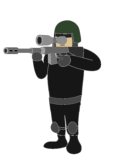
\includegraphics[scale=0.5]{asset/image/sniper_eu.png}
    \caption{Une autre unité qui attaque à distance}
    \end{figure}

\section{Annexe \& Source}
\begin{itemize}
    \item Le pseudocode de la grille par hexagone : \url{https://www.redblobgames.com/grids/hexagons/}
    \item La musique du jeu : \url{https://soundcloud.com/leagueoflegends/omega-squad-teemo}
    \item Les dessins ont été faits avec Illustrator \url{https://www.adobe.com/products/illustrator.html}
\end{itemize}
\subsection{Contact}
\begin{itemize}
    \item nguyenthiet.lam@gmail.com
    \item lam.nguyen-thiet@u-psud.fr
    \item kenyu.kobayashi@u-psud.fr
\end{itemize}


\end{document}
